
%%%%%%%%%%%%%%%%%%%%%%%%%%%%%%%%%%%%%%%%%%%%%%%%%%%%%%%%%%%%%%%%%%%%%%%%%%%%%%
% Copyright (c) 2003-2014 by University of Queensland
% http://www.uq.edu.au
%
% Primary Business: Queensland, Australia
% Licensed under the Open Software License version 3.0
% http://www.opensource.org/licenses/osl-3.0.php
%
% Development until 2012 by Earth Systems Science Computational Center (ESSCC)
% Development 2012-2013 by School of Earth Sciences
% Development from 2014 by Centre for Geoscience Computing (GeoComp)
%
%%%%%%%%%%%%%%%%%%%%%%%%%%%%%%%%%%%%%%%%%%%%%%%%%%%%%%%%%%%%%%%%%%%%%%%%%%%%%%

\section{Example 5: A Heat Refraction Model}
\label{example5}
\sslist{example05a.py and cblib.py}
Our heat refraction model will be a large anticlinal structure that is subject
to a constant temperature at the surface and experiencing a steady heat flux at
its base. Our aim is to show that the temperature flux across the surface is
not linear from bottom to top, but is in fact warped by the structure of the
model. The heat flow pattern demonstrates the dependence upon the material
properties and the shape of the interface.

The script of \refSec{example4} is modified by subdividing the block into two
parts. The curve separating the two blocks is given as a spline, see
\reffig{fig:anticlinehrmodel}. The data points
used to define the curve may be imported from a database of measurements
(\textit{e.g.} borehole depth data), but for simplicity it is assumed here that
the coordinates are known in an analytic form.

\begin{figure}[ht]
\centerline{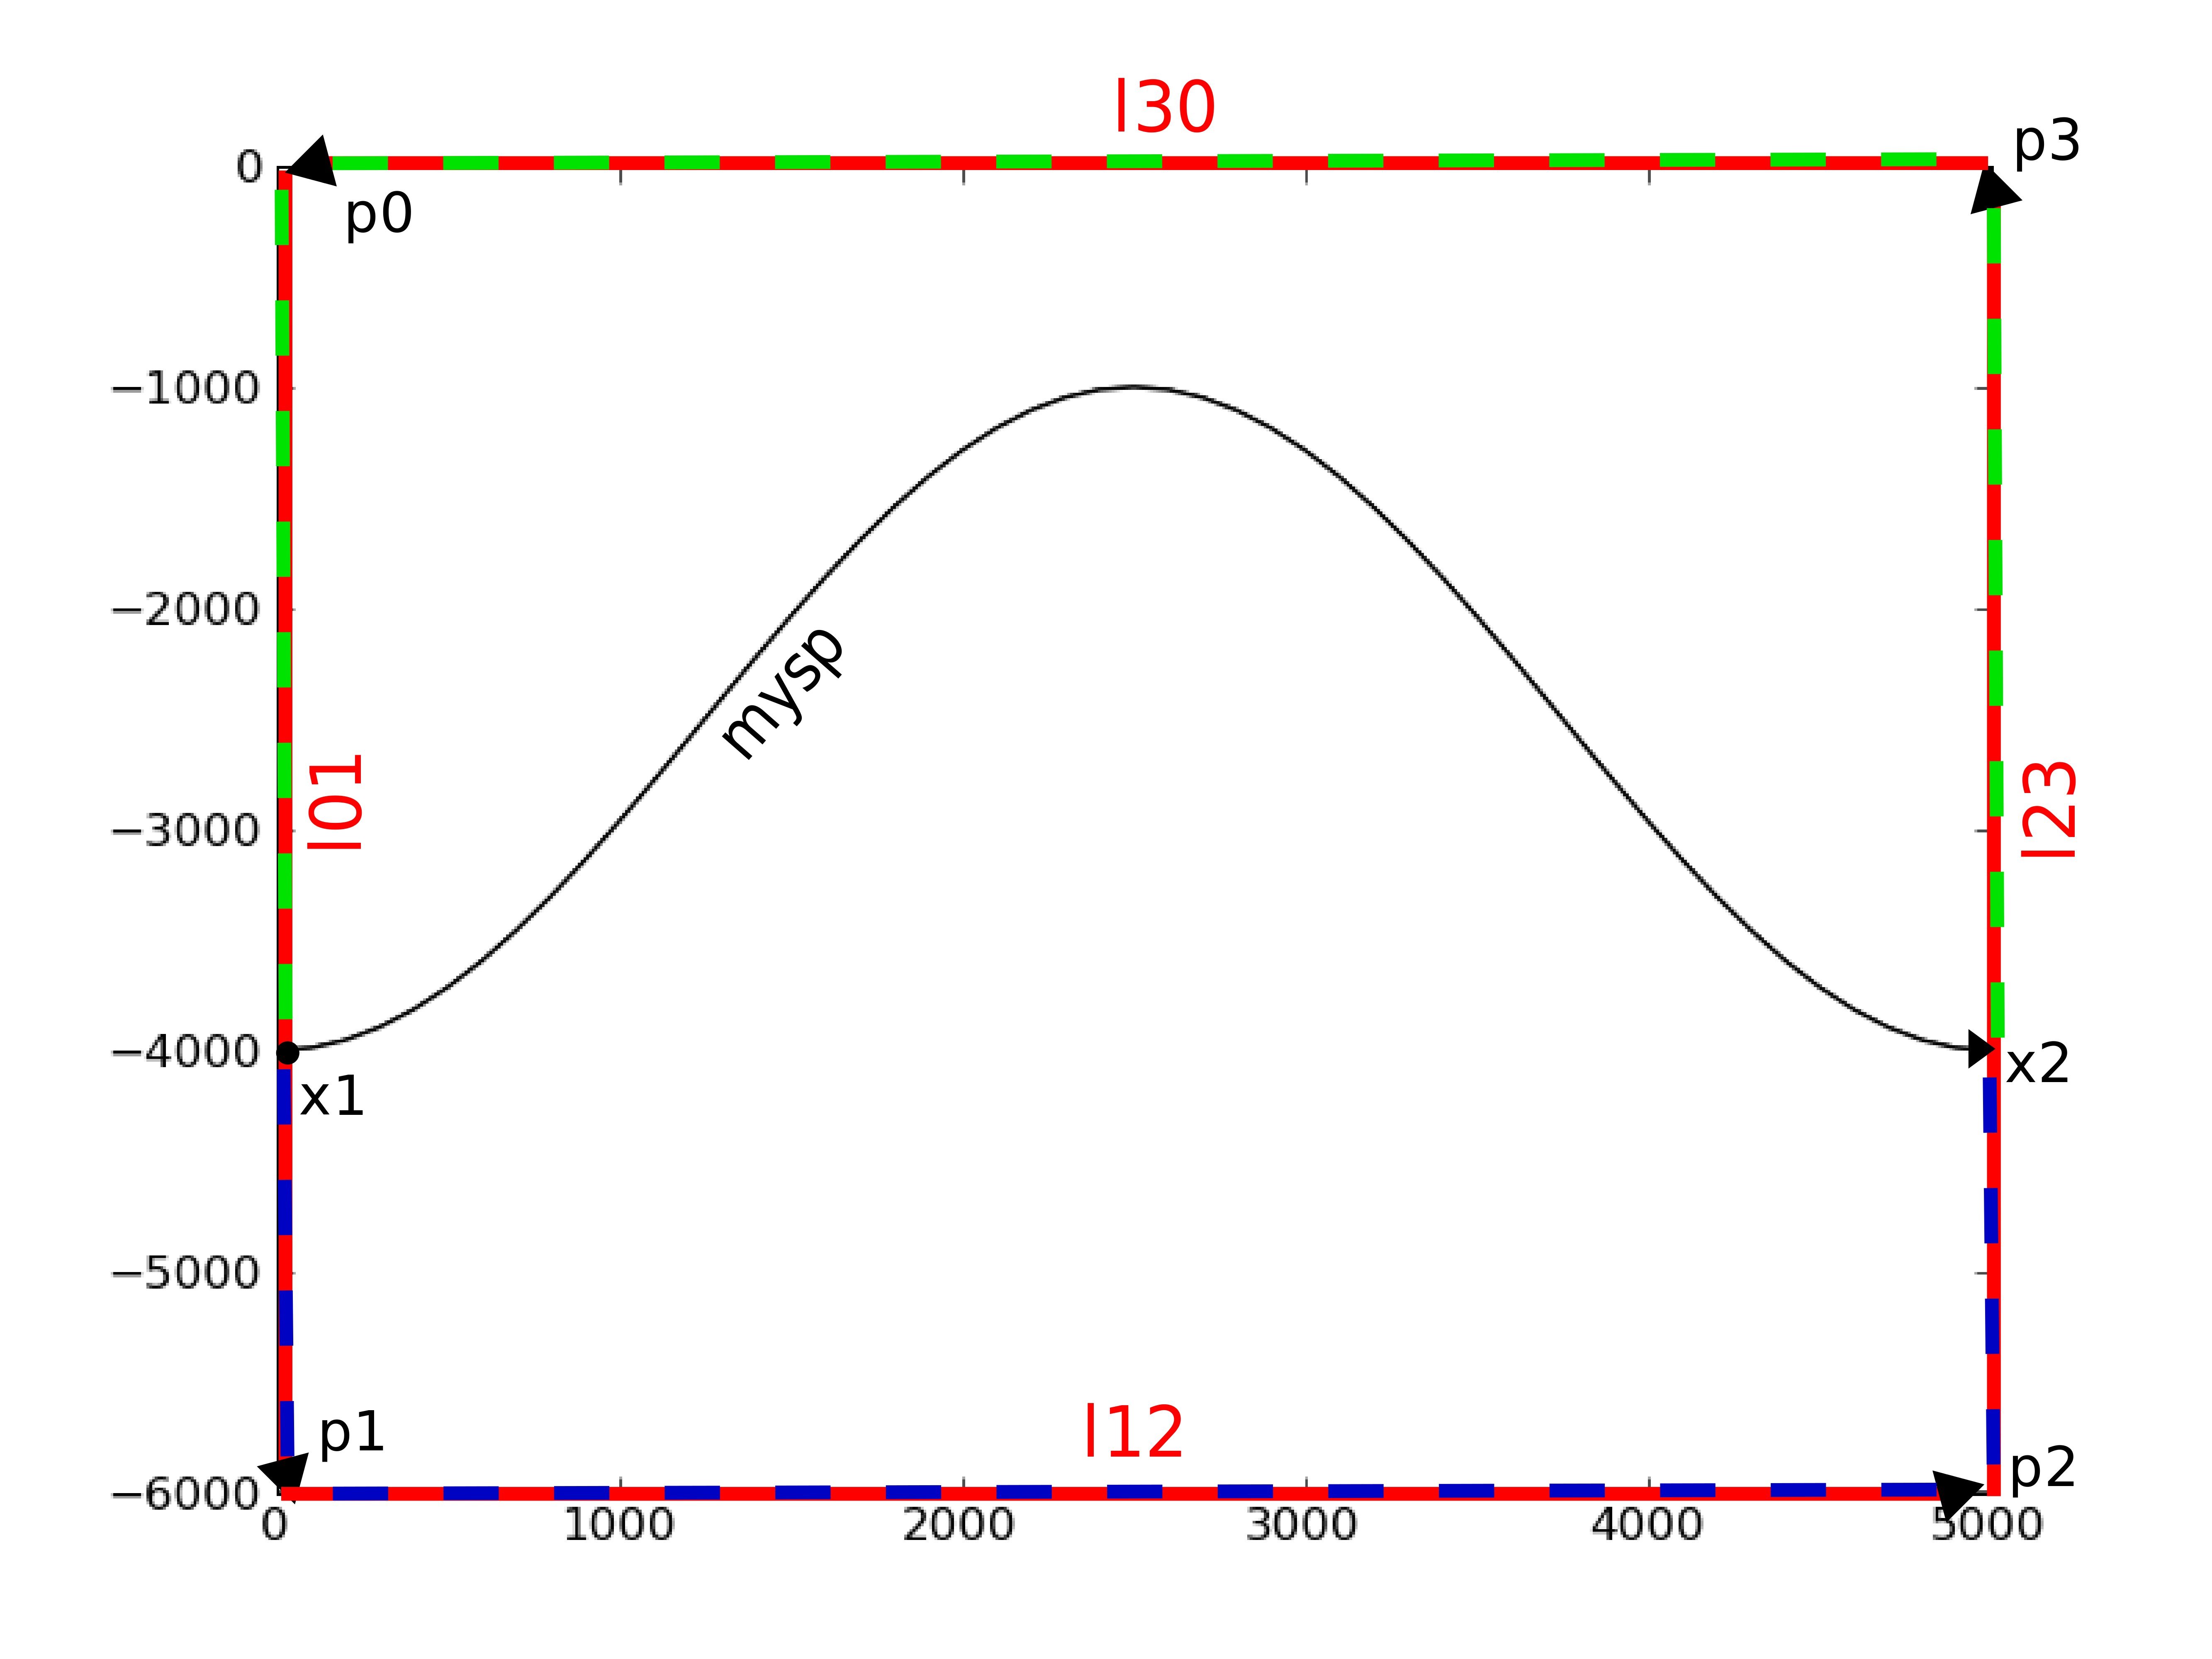
\includegraphics[width=4.in]{figures/anticlineheatrefraction.png}}
\caption{Example 5a: Heat refraction model with point and line labels}
\label{fig:anticlinehrmodel}
\end{figure}

There are two modes available in this example. When \verb|modal=1|, this
indicates to the script that the model should be an anticline. Otherwise, when
\verb|modal=-1|, the model is a syncline. The modal operator simply changes the
orientation of the boundary function so that it is either upwards or downwards
curving. A \verb|save_path| has also been defined so that we can easily separate
our data from other examples and our scripts. 

It is now possible to start defining our domain and boundaries. 

The curve defining our clinal structure is located approximately in the middle
of the domain and has a sinusoidal shape. We define the curve by generating
points at discrete intervals; $51$ in this case, and then create a smooth curve
through the points using the \verb|Spline()| function.
\begin{python}
# Material Boundary
x=[ Point(i*dsp\
    ,-dep_sp+modal*orit*h_sp*cos(pi*i*dsp/dep_sp+pi))\
     for i in range(0,sspl)\
    ]
mysp = Spline(*tuple(x)) #*tuple() forces x to become a tuple
\end{python}
The start and end points of the spline can be returned to help define the
material boundaries.
\begin{python}
x1=mysp.getStartPoint()
x2=mysp.getEndPoint()
\end{python}
The top block or material above the clinal/spline boundary is defined in an
\textbf{anti-clockwise} manner by creating lines and then a closed loop. By
meshing the sub-domain we also need to assign it a planar surface. 
\begin{python}
# TOP BLOCK
tbl1=Line(p0,x1)
tbl2=mysp
tbl3=Line(x2,p3)
l30=Line(p3, p0)
tblockloop = CurveLoop(tbl1,tbl2,tbl3,l30)
tblock = PlaneSurface(tblockloop)
\end{python}
This process is repeated for every other sub-domain. In this example there is
only one other, the bottom block. The process is similar to the top block but
with a few differences. The spline points must be reversed by setting the spline
as negative.
\begin{python}
bbl4=-mysp
\end{python}
This reverse spline option unfortunately does not work for the
\verb|getLoopCoords| command, however, the \modmpl polygon tool will accept
clock-wise oriented points so we can define a new curve.
\begin{python}
#clockwise check
bblockloop=CurveLoop(mysp,Line(x2,p2),Line(p2,p1),Line(p1,x1))
\end{python}
The last few steps in creating the domain require that the previously defined
domain and sub-domain points are submitted to generate a mesh that can be
imported into \esc.
To initialise the mesh it first needs some design parameters. In this case we
have 2 dimensions \verb|dim| and a specified number of finite elements that need
to be applied to the domain \verb|element_size|. It then becomes a simple task
of adding the sub-domains and flux boundaries to the design. Each element of our
model can be given an identifier which makes it easier to define the sub-domain
properties in the solution script. This is done using the 
\verb|PropertySet()| function. The geometry and mesh are then saved so the
\esc domain can be created.
\begin{python}
# Create a Design which can make the mesh
d=Design(dim=2, element_size=200)
# Add the sub-domains and flux boundaries.
d.addItems(PropertySet("top",tblock),PropertySet("bottom",bblock),\
                   PropertySet("linebottom",l12))
# Create the geometry, mesh and escript domain
d.setScriptFileName(os.path.join(save_path,"example05.geo"))
d.setMeshFileName(os.path.join(save_path,"example05.msh"))
domain=MakeDomain(d,optimizeLabeling=True)
\end{python}
The creation of our domain and its mesh is now complete.

With the mesh imported it is now possible to use our tagging property to set up
our PDE coefficients. In this case $\kappa$ is set via the
\verb|setTaggedValue()| function which takes two arguments, the name of the
tagged points and the value to assign to them. 
\begin{python}
# set up kappa (thermal conductivity across domain) using tags
kappa=Scalar(0,Function(domain))
kappa.setTaggedValue("top",2.0*W/m/K)
kappa.setTaggedValue("bottom",4.0*W/m/K)
\end{python}
No further changes are required to the PDE solution step, see
\reffig{fig:anticlinetemp} for the result. 

\begin{figure}[ht]
\centerline{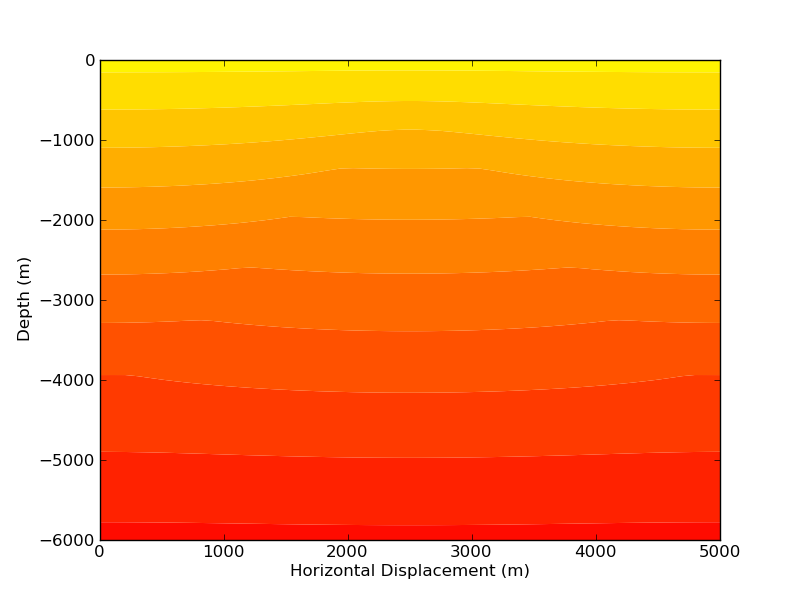
\includegraphics[width=4.in]{figures/heatrefraction}}
\caption{Example 5a: Temperature Distribution in the Heat Refraction Model}
\label{fig:anticlinetemp}
\end{figure}
\clearpage

\section{Line Profiles of 2D Data}
\sslist{example05b.py and cblib.py}
We want to investigate the profile of the data of the last example. 
Of particular interest is the depth profile of the heat flux which is the
second component of $-\kappa \nabla T$. The script from the previous section
is extended to show how a vertical profile can be plotted.

The first important piece of information, is that \esc assumes that $-\kappa
\nabla T$ is not smooth and that the point values of this solution are defined
at numerical interpolation points. This assumption is reasonable as
the flux is the product of the piecewise constant function $\kappa$ and 
the gradient of the temperature $T$ which has a discontinuity at the rock
interface.
Before plotting this function we need to smooth the solution using the
\verb|Projector()| class;
\begin{python}
from esys.escript.pdetools import Projector
proj=Projector(domain)
qu=proj(-kappa*grad(T))
\end{python}
The \verb|proj| object provides a mechanism to distribute values given at the
numerical interpolation points to the nodes of the FEM mesh - the heat flux in
this example. \verb|qu| has the same function space as the temperature
\verb|T|. The smoothed flux is interpolated to a regular $200\times 200$ grid
via;
\begin{python}
xiq,yiq,ziq = toRegGrid(qu[1],200,200)
\end{python}
using the \verb|toRegGrid| function from the cookbook library which we are
using for the contour plot.
At return \verb|ziq[j,i]| is the value of vertical heat flux at point
(\verb|xiq[i]|,\verb|yiq[j]|). We can easily create deep profiles now by
plotting slices \verb|ziq[:,i]| over \verb|yiq|. The following script
creates a deep profile at $x_{0}=\frac{width}{2}$;
\begin{python}
cut=int(len(xiq)/2)
pl.plot(ziq[:,cut]*1000.,yiq)
pl.title("Vertical Heat Flow Depth Profile")
pl.xlabel("Heat Flow (mW/m^2)")
pl.ylabel("Depth (m)")
pl.savefig(os.path.join(save_path,"hf.png"))
\end{python}
This process can be repeated for various variations of the solution.
\reffig{figs:dps} shows temperature, temperature gradient, thermal conductivity
and heat flow.

\begin{figure}[htp]
\centering
    \subfigure[Temperature Depth
Profile]{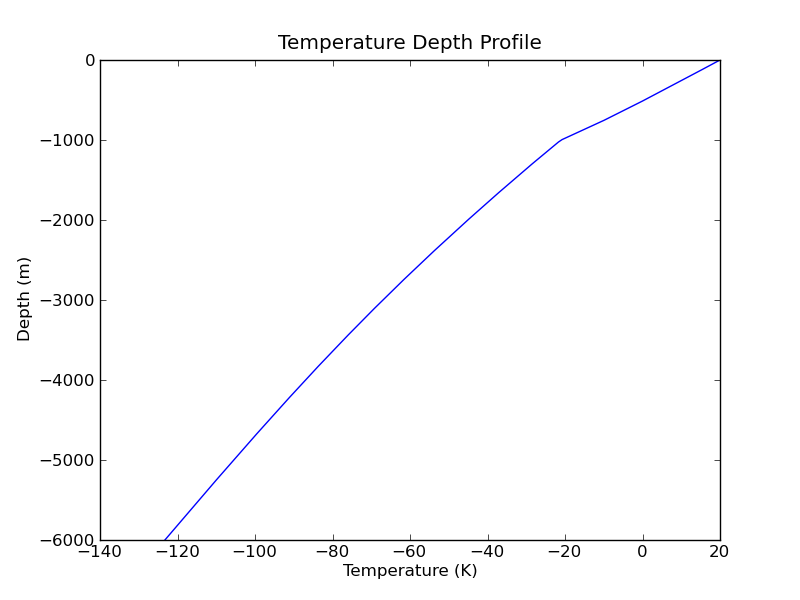
\includegraphics[width=3in]{figures/heatrefractiontdp.png}\label{
fig:tdp}}
    \subfigure[Temperature Gradient Depth
Profile]{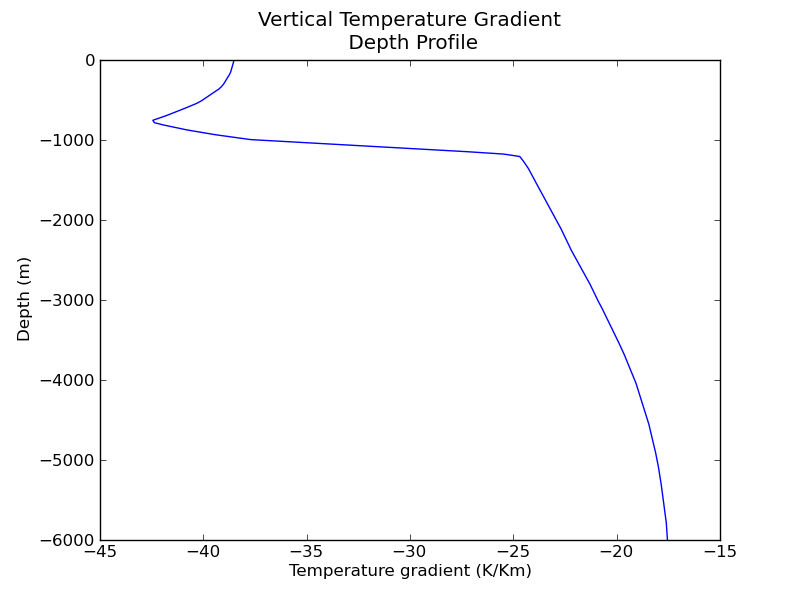
\includegraphics[width=3in]{figures/heatrefractiontgdp.png}\label{
fig:tgdp}}
    \subfigure[Thermal Conductivity
Profile]{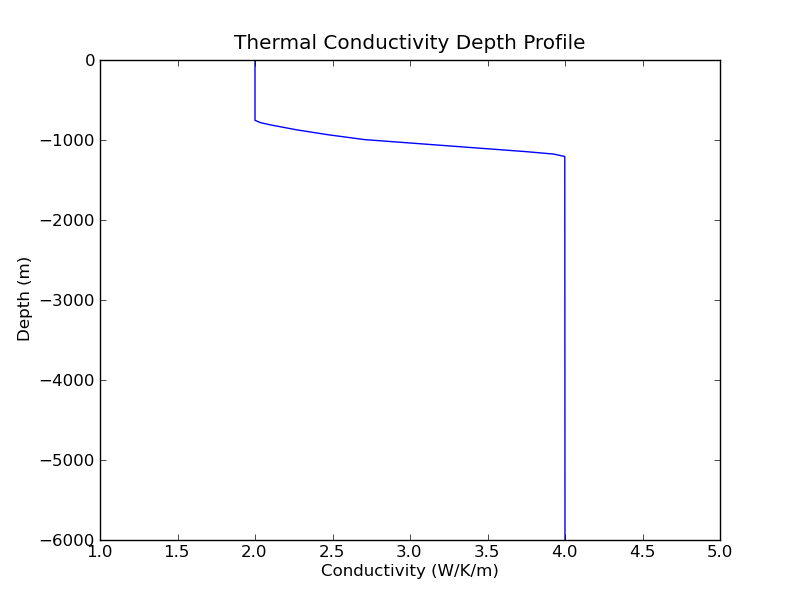
\includegraphics[width=3in]{figures/heatrefractiontcdp.png}\label{
fig:tcdp}}
    \subfigure[Heat Flow Depth
Profile]{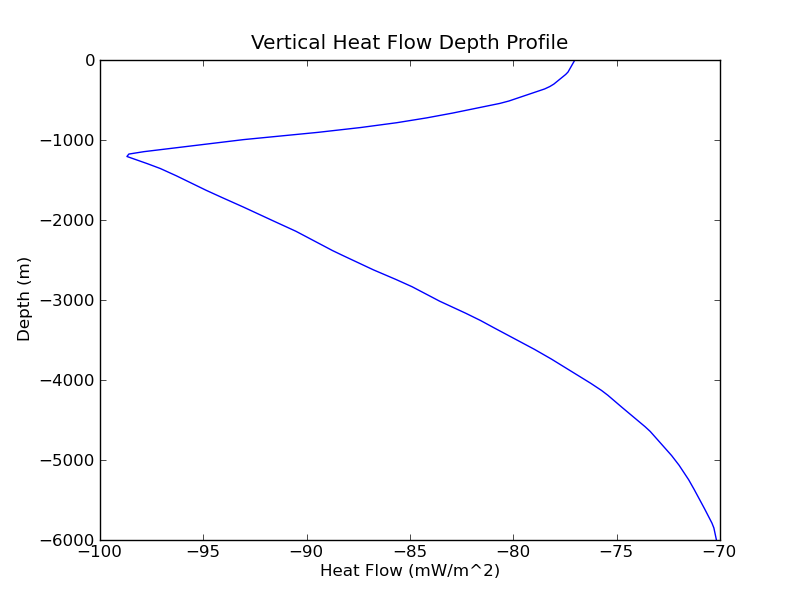
\includegraphics[width=3in]{figures/heatrefractionhf.png}\label{fig:hf}
}
  \caption{Example 5b: Depth profiles down centre of model}
  \label{figs:dps}
\end{figure}
\clearpage

\section{Arrow Plots in \mpl}
\sslist{example05c.py and cblib.py}
The distribution of the flux $-\kappa \nabla T$ is now visualised over the
domain and the results are plotted in \reffig{fig:hr001qumodel}. 
The plot puts together three components. A contour plot of the temperature,
a coloured representation of the two sub-domains where colour represents the
thermal conductivity in the particular region, and finally the arrows
representing the local direction of the steepest gradient of the flux.

Contours have already been discussed in \refSec{Sec:2DHD plot}. To show
sub-domains, we need to go back to \pycad data to get the points used to
describe the boundary of the sub-domains. We have created the \verb|CurveLoop|
class object \verb|tblockloop| to define the boundary of the upper sub-domain.
We use the \verb|getPolygon()| method of \verb|CurveLoop| to get
access to the \verb|Point|s used to define the boundary. The statement
\begin{python}
[ p.getCoordinates() for p in tblockloop.getPolygon() ]
\end{python}
creates a list of the node coordinates of all the points in question. In order 
to simplify the selection of the $x$ and $y$ coordinates the list is converted 
into \modnumpy array. To add the area coloured in brown to the plot we use; 
\begin{python}
import pylab as pl
import numarray as np
tpg=np.array([p.getCoordinates() for p in tblockloop.getPolygon() ])
pl.fill(tpg[:,0],tpg[:,1],'brown',label='2 W/m/k',zorder=-1000)
\end{python}
The same code is applied to \verb|bblockloop| to create the red area for this
sub-domain.

To plot vectors representing the flux orientation we use the 
\verb|quiver| function in \pylab. The function places vectors at locations in
the domain.
For instance one can plot vectors at the locations of the sample points used by
\esc to represent the flux \verb|-kappa*grad(T)|. As a vector is plotted at
each sample point one typically ends up with too many vectors. So one needs to
select a subset of points as follows:

First we create a coarse grid of points on a rectangular mesh, e.g. $20 \times
20$ points. Here we choose a grid of points which are located at the centre of
a \verb|nx| $\times$ \verb|ny| grid;
\begin{python}
dx = width/nx # x spacing
dy = depth/ny # y spacing
grid = [ ] # the grid points
for j in range(0,ny-1):
    for i in range(0,nx-1):
           grid.append([dx/2+dx*i,dy/2+dy*j])
\end{python}
With the \verb|Locator| function \esc provides a mechanism to identify sample
points that are closest to the grid points we have selected and to retrieve the
data at these points; 
\begin{python}
from esys.escript.pdetools import Locator
flux=-kappa*grad(T)
fluxLoc = Locator(flux.getFunctionSpace(),grid)
subflux= fluxLoc(flux) 
\end{python}
\verb|subflux| now contains a list of flux components at certain sample points.
To get the list of the sample point coordinates one can use the \verb|getX()|
method of the \verb|Locator|;
\begin{python}
subfluxloc = fluxLoc.getX()
\end{python}
To simplify the selection of $x$ and $y$ components it is convenient to
transform \verb|subflux| and \verb|subfluxloc| to \numpy arrays
\verb|xflux|, \verb|flux|.
This function is implemented in the \verb|subsample| function within the
\file{clib.py} file so we can use it in other examples. One can easily use this
function to create a vector plot of the flux;
\begin{python}
from cblib import subsample
xflux, flux=subsample(-kappa*grad(T), nx=20, ny=20)
pl.quiver(xflux[:,0],xflux[:,1],flux[:,0],flux[:,1], angles='xy',color="white")
\end{python}
Finally, we add a title and labels;
\begin{python}
pl.title("Heat Refraction across a clinal structure.")
pl.xlabel("Horizontal Displacement (m)")
pl.ylabel("Depth (m)")
pl.title("Heat Refraction across a clinal structure \n with gradient quivers.")
pl.savefig(os.path.join(saved_path,"flux.png"))
\end{python} 
to get the desired result, see \reffig{fig:hr001qumodel}.

\begin{figure}[ht]
\centerline{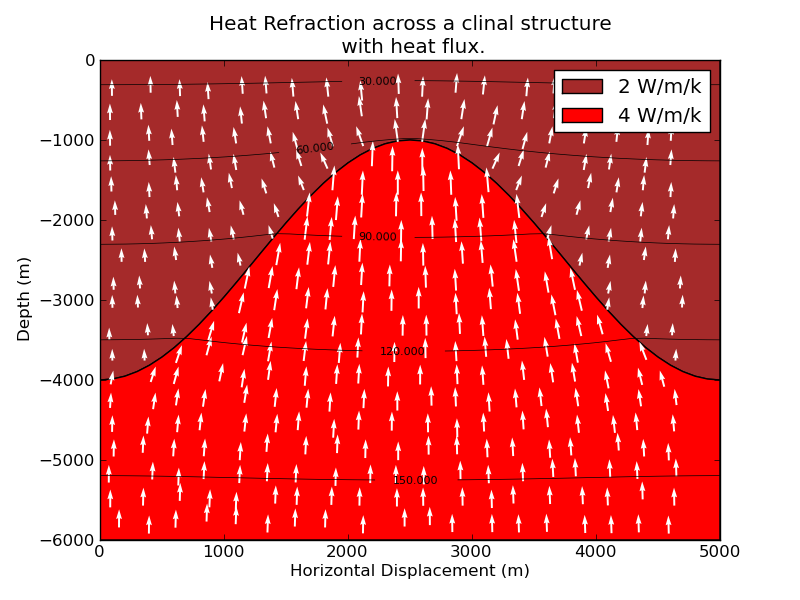
\includegraphics[width=5.in]{figures/heatrefractionflux}}
\caption{Example 5c: Heat refraction model with gradient indicated by vectors}
\label{fig:hr001qumodel}
\end{figure}
\clearpage

\section{Example 6:Fault and Overburden Model}
\sslist{example06.py and cblib.py}
A slightly more complicated model can be found in the example file
\textit{heatrefraction2_solver.py} where three blocks are used within the
model, see~\reffig{fig:hr002qumodel}. It is left to the reader to work through
this example.

\begin{figure}[ht]
\centerline{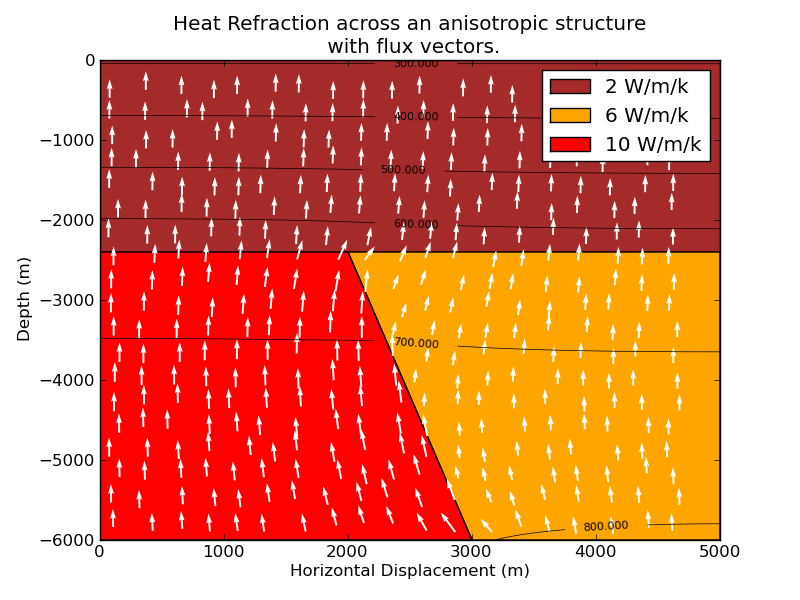
\includegraphics[width=4.in]{figures/heatrefraction2flux}}
\caption{Example 6: Heat refraction model with three blocks and heat flux}
\label{fig:hr002qumodel}
\end{figure}
\clearpage
